\begin{figure*}[t]
	\centering
	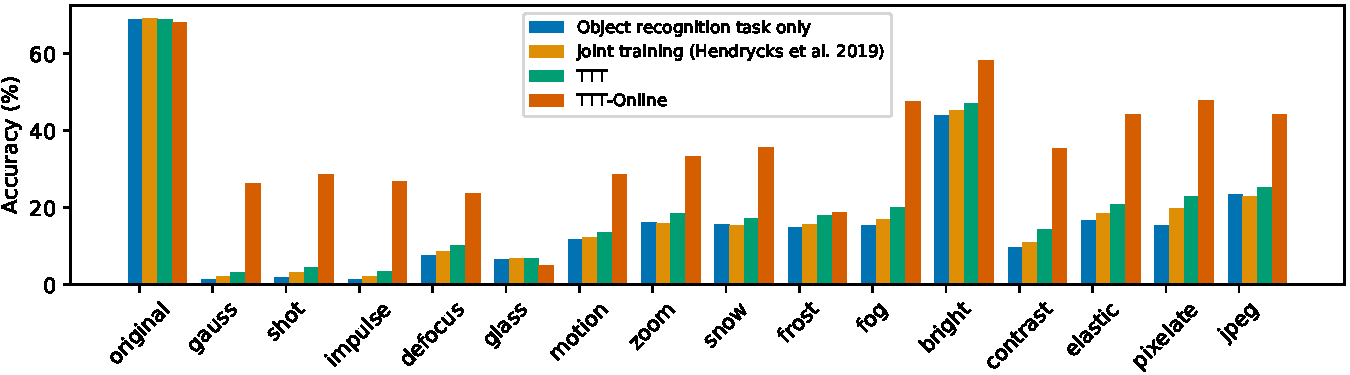
\includegraphics[width=1.0\textwidth]{plots/test_layer3_5_gn}
		\vspace{-2ex}
	\begin{subfigure}[b]{1.0\textwidth}
		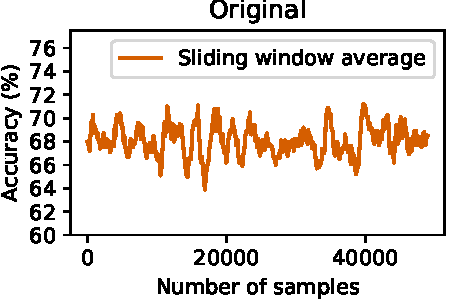
\includegraphics[width=0.325\textwidth]{plots/online_curves/original_5_avg}
		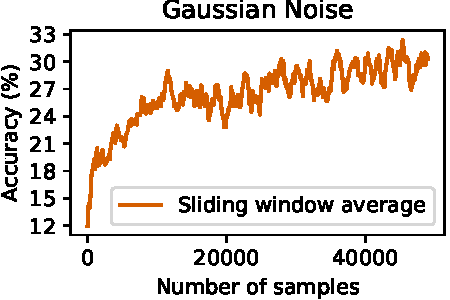
\includegraphics[width=0.325\textwidth]{plots/online_curves/gaussian_noise_5_avg}
		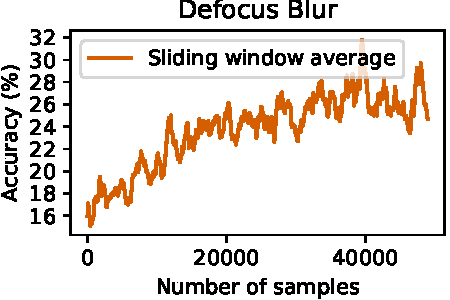
\includegraphics[width=0.325\textwidth]{plots/online_curves/defocus_blur_5_avg}
	\end{subfigure}
	\begin{subfigure}[b]{1.0\textwidth}
			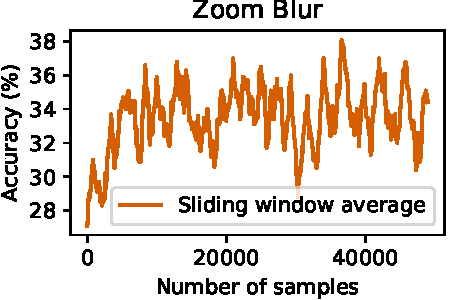
\includegraphics[width=0.325\textwidth]{plots/online_curves/zoom_blur_5_avg}
			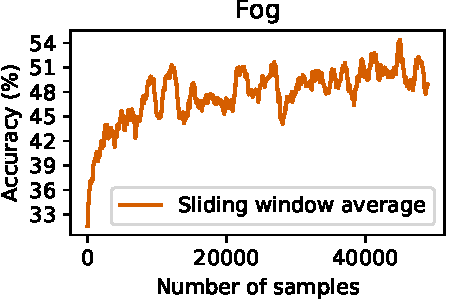
\includegraphics[width=0.325\textwidth]{plots/online_curves/fog_5_avg}
			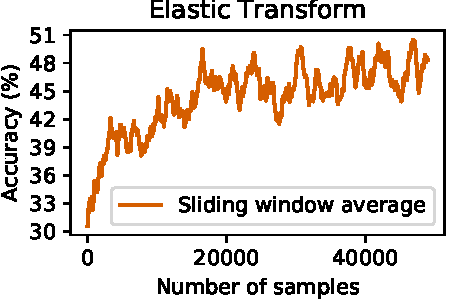
\includegraphics[width=0.325\textwidth]{plots/online_curves/elastic_transform_5_avg}
	\end{subfigure}
	\caption{
		{\bf Test accuracy (\%) on ImageNet-C with level 5 corruptions.} Upper panel: Our approaches, TTT and TTT-Online, show significant improvements in all corruption types over the two baselines. 
		Lower panel: We show the accuracy of TTT-Online as the average over a sliding window of 100 samples; TTT-Online generalizes better as more samples are evaluated (x-axis), without hurting on the original distribution. We use accuracy instead of error here because the baseline performance is very low for most corruptions.
	}
	\label{fig:cc_imagenet}
	\vspace{-1ex}
\end{figure*}